\documentclass[twoside,12pt]{book}
\usepackage{setspace}
\setstretch{1.25}
\usepackage[square, sort, numbers, authoryear]{natbib}
\usepackage{amsmath}

\title{Surface Flux Transport Model User Manual}

\begin{document}
\maketitle

\chapter{The Basics \label{chapter:basics}}

\section{Magnetic field evolution on the solar surface}


The surface flux transport (SFT) model, which solves the radial component of the magnetic field on the solar surface, has demonstrated remarkable effectiveness in simulating the dynamics of the large-scale magnetic field on the photosphere. The governing equation can be written as,

\begin{equation}
\frac{\partial B}{\partial t} = \frac{D}{R_\odot^2}\left[\frac{\partial}{\partial s}\left((1-s^2)\frac{\partial B}{\partial s}\right) + \frac{1}{1-s^2}\frac{\partial^2B}{\partial\phi^2}\right] - \frac{\partial}{\partial s}\left[\frac{v_s(s)}{R_\odot}\sqrt{1-s^2} B\right]- \Omega(s)\frac{\partial B}{\partial\phi},
\end{equation}
where $s =$ sin$\theta$, $D$ is the magnetic diffusivity, $\Omega (s)$ is the angular velocity in east-west direction on a sine-latitude grid, $v_s (s)$ is the flow profile along north-south direction on a sine-latitude grid and $\phi$ is the longitude. As the velocity profiles involved in transporting the magnetic flux on the photosphere is a function of latitude only, we can simplify this equation by taking average in the longitudinal direction which will improve the computational efficiency and provide us a lesser parameter space to comprehensively explore the dynamics. After averaging the $B_r$, 
\begin{equation}
\overline{B}(s,t)=(2\pi)^{-1}\int_0^{2\pi}B(s,\phi,t)\,\mathrm{d}\phi.
\end{equation}
Using this reduced form of $B_r$, we can re-write equation-\ref{eqn:sft2d} as,
\begin{equation}
\frac{\partial\overline{B}}{\partial t} = \frac{\partial}{\partial s}\left[\frac{D}{R_\odot^2}(1-s^2)\frac{\partial\overline{B}}{\partial s} - \frac{v_s(s)}{R_\odot}\sqrt{1-s^2}\overline{B}\right],
\end{equation}
where the north-south velocity is,
\begin{equation}
v_s(s) = D_us(1-s^2)^{p/2}.
\end{equation}
In this form the velocity, $s =$ sin$\theta$ and $D_u$ controls the amplitude of the function. 

\begin{figure}
    \centering
    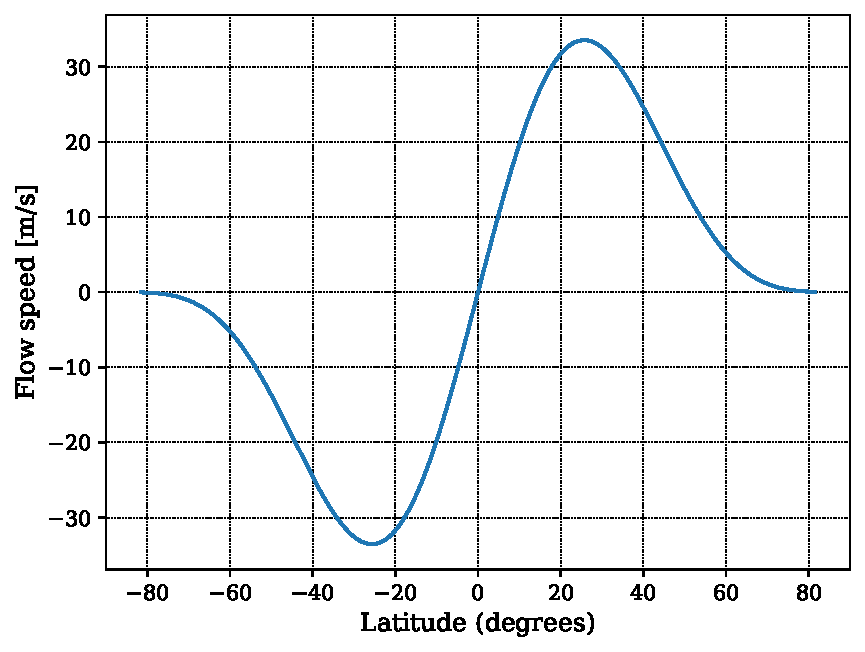
\includegraphics[width=0.7\textwidth]{assets/MC_flow250.pdf}
    \caption{Example flow profile in the north-south direction using equation-\ref{eqn:merid}.}
\end{figure}
Presently the code solves equation-\ref{eqn:evol} on a sine latitude grid, figure-\ref{fig:grid} shows an example of the grid point distribution on a ($s$,$\phi$) grid containing (10,20) points.
\begin{figure}[htbp]
    \centering
    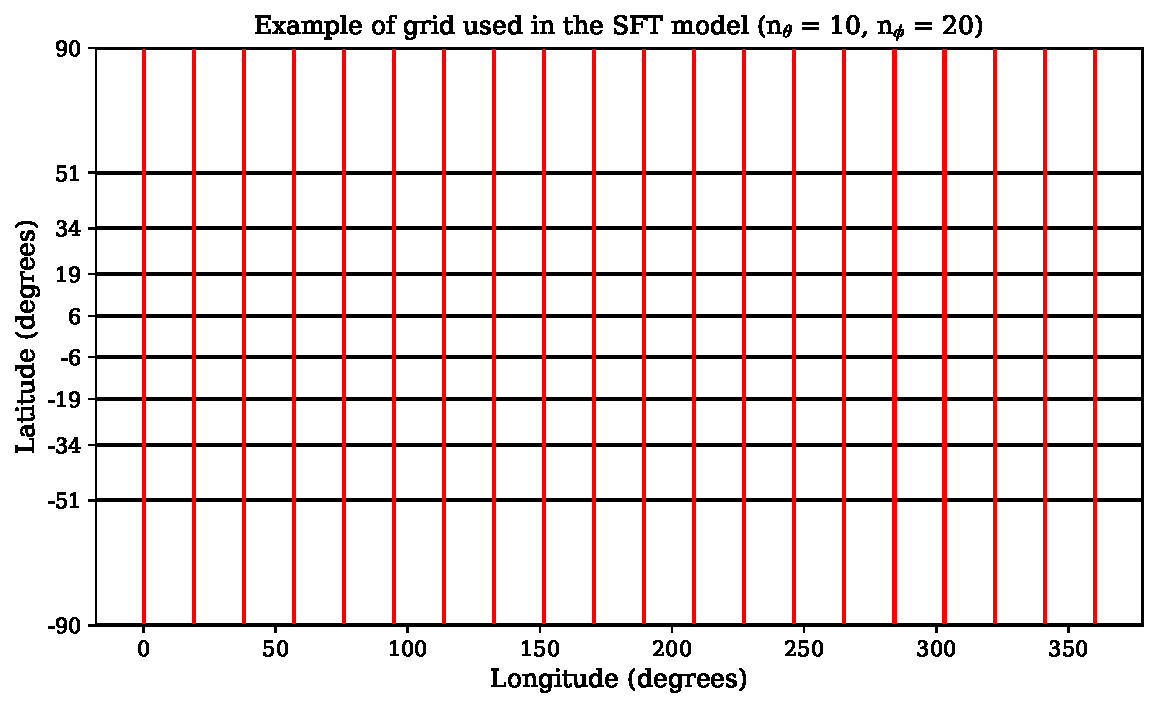
\includegraphics[width=0.85\textwidth]{assets/grid_structure_sft1D.pdf}
    \caption{Example grid visualization with 10, 20 points in sine latitude ($s$) and longitude ($\phi$ direction respectively.}
\end{figure}
\subsection{Bipolar approximation}
We introduce a source function to model the approximating bipolar magnetic region (BMR) for an observed SHARP. The location of the center of the BMR we use the locations of the positive and negative polarity positions $(s_+, \phi_+)$ and $(s_-,\phi_-)$ on the computational grid. Here $s$ denotes sine-latitude and $\phi$ denotes (Carrington) longitude. We compute,
\begin{itemize}
    \Item centroid of the BMR,\\ \\ \begin{align}
    s_0 = \frac12(s_+ + s_-),\qquad \phi_0 = \frac12(\phi_+ + \phi_-)
    \end {align}
    \Item polarity separation, which is the heliographic angle,\\ \\ \begin{align}
    \rho = \arccos\left[s_+s_- + \sqrt{1-s_+^2}\sqrt{1 - s_-^2}\cos(\phi_+-\phi_-) \right]
    \end {align}
    \Item the tilt angle with respect to the equator, given by,\\ \\ \begin{align}
    \gamma = \arctan\left[\frac{\arcsin(s_+) - \arcsin(s_-)}{\sqrt{1-s_0^2}(\phi_- - \phi_+)}\right]
    \end {align}
\end{itemize}


Together with the unsigned flux, $|\Phi|$, these parameters define the BMR for our chosen functional form. For an untilted BMR centered at $s=\phi=0$, this functional form is defined as
\begin{equation}
B(s,\phi) = F(s,\phi) = -B_0\frac{\phi}{\rho}\exp\left[-\frac{\phi^2 + 2\arcsin^2(s)}{(a\rho)^2}\right],
\end{equation}
where the amplitude $B_0$ is scaled to match the corrected flux of the observed region on the computational grid. To account for the location $(s_0,\phi_0)$ and tilt $\gamma$ of a general region, we set $B(s,\phi) = F(s',\phi')$, where $(s',\phi')$ are spherical coordinates in a frame where the region is centered at $s'=\phi'=0$ and untilted. Figure \ref{fig:example-bmr} shows an example BMR.

\begin{figure}
    \centering
    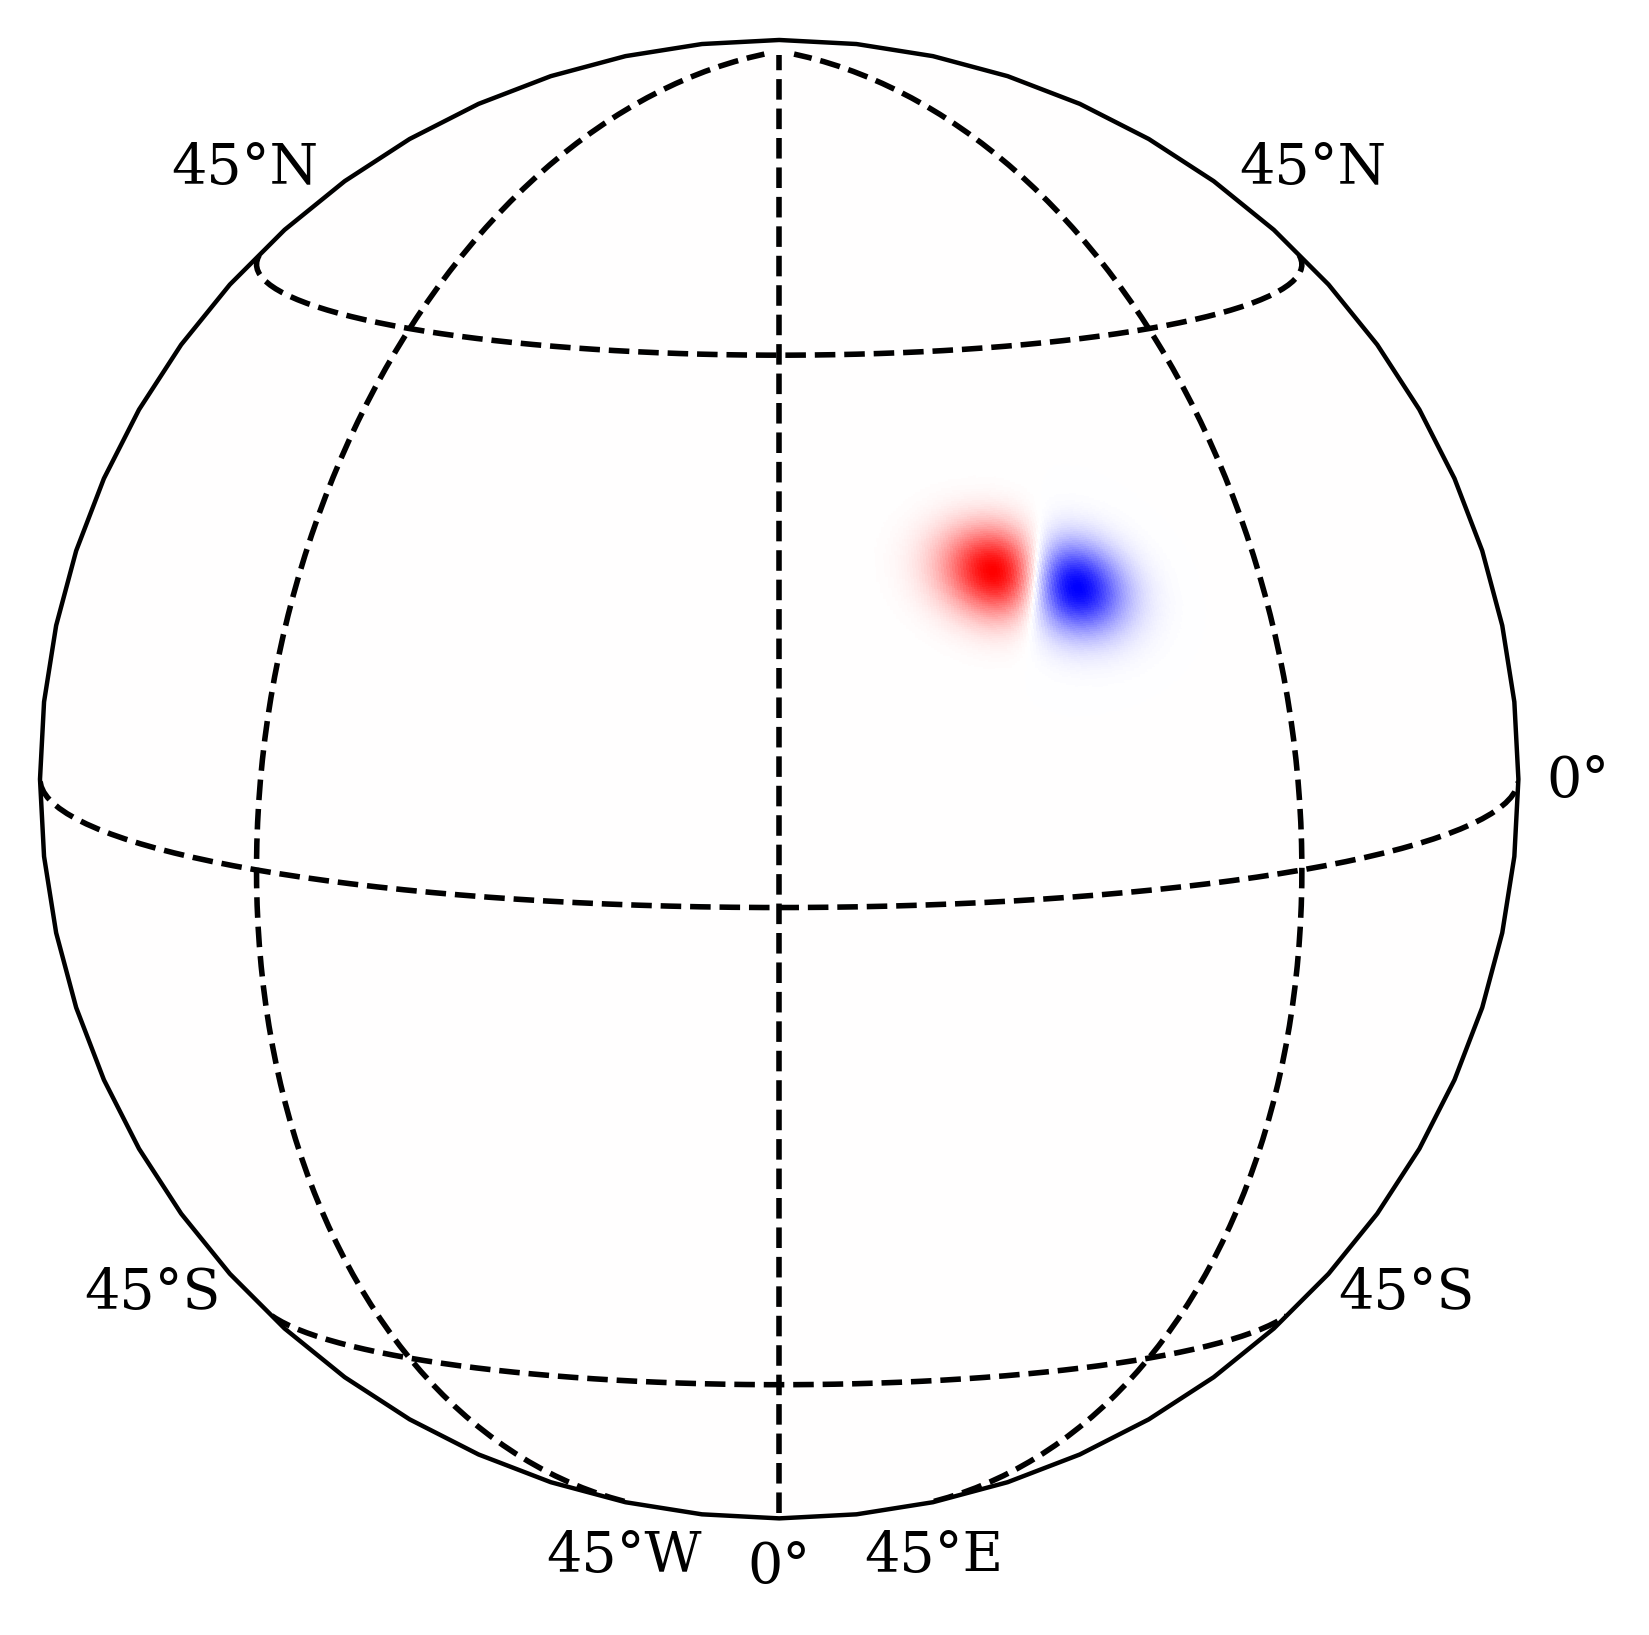
\includegraphics[width=0.5\textwidth]{assets/example_bmr.png}
    \caption{A BMR centered at 25$^{\circ}$ latitude and 22.5$^{\circ}$ longitude with a tilt of 30$^{\circ}$ with respect to the equator calculated using equation-\ref{eqn:bmr}}
\end{figure}
\subsection{Coordinate transformation}
The coordinate transformation from the frame $(s,\phi)$ where the BMR is centred at $s=\phi=0$ to the frame $(s',\phi')$ where it is centred at $(s_0,\phi_0)$ with tilt $\gamma$. This amounts to a rotation, which is easiest to express in Cartesian coordinates
\begin{equation}
x = \cos\phi\sqrt{1-s^2}, \quad y=\sin\phi\sqrt{1-s^2},\quad z=s.
\end{equation}
Multiplying by the rotation matrices for the sequence of rotations indicated in Figure \ref{fig:rotation-bmr} shows that Cartesian coordinates in the rotated frame are
\begin{eqnarray}\nonumber
\left[
\begin{array}{c}
x'\\
y'\\
z'
\end{array}
\right] &=&
\left[
\begin{array}{ccc}
1\; & 0\; & 0\\
0\; & \cos\gamma\; & -\sin\gamma\\
0\; & \sin\gamma\; & \cos\gamma
\end{array}
\right]
\left[
\begin{array}{ccc}
\cos\lambda_0\; & 0\; & \sin\lambda_0\\
0\; & 1\; & 0\\
-\sin\lambda_0\; & 0\; & \cos\lambda_0
\end{array}
\right]
\cdot\\ 
&&\cdot
\left[
\begin{array}{ccc}
\cos\phi_0\; & \sin\phi_0\; & 0\\
-\sin\phi_0\; & \cos\phi_0\; & 0\\
0 & 0 & 1
\end{array}
\right]
\left[
\begin{array}{c}
x\\
y\\
z
\end{array}
\right],
\end{eqnarray}
where $s_0=\sin\lambda_0$. From these we determine $\phi'=\arctan(y'/x')$ and $s' = z'$.

The parameter $a$ in equation-\ref{eqn:bmr} controls the size of the BMR relative to the separation, $\rho$, of the original polarity centroids. For given values of $\lambda_0$, $\gamma$, and $\rho$, and $B_0$ chosen to give the required magnetic flux, the parameter $a$ may be chosen to control the axial dipole moment of the BMR. A good match to the axial dipole moment of the original SHARP is obtained with $a=0.56$, and the same value works for every region.

\begin{figure}
    \centering
    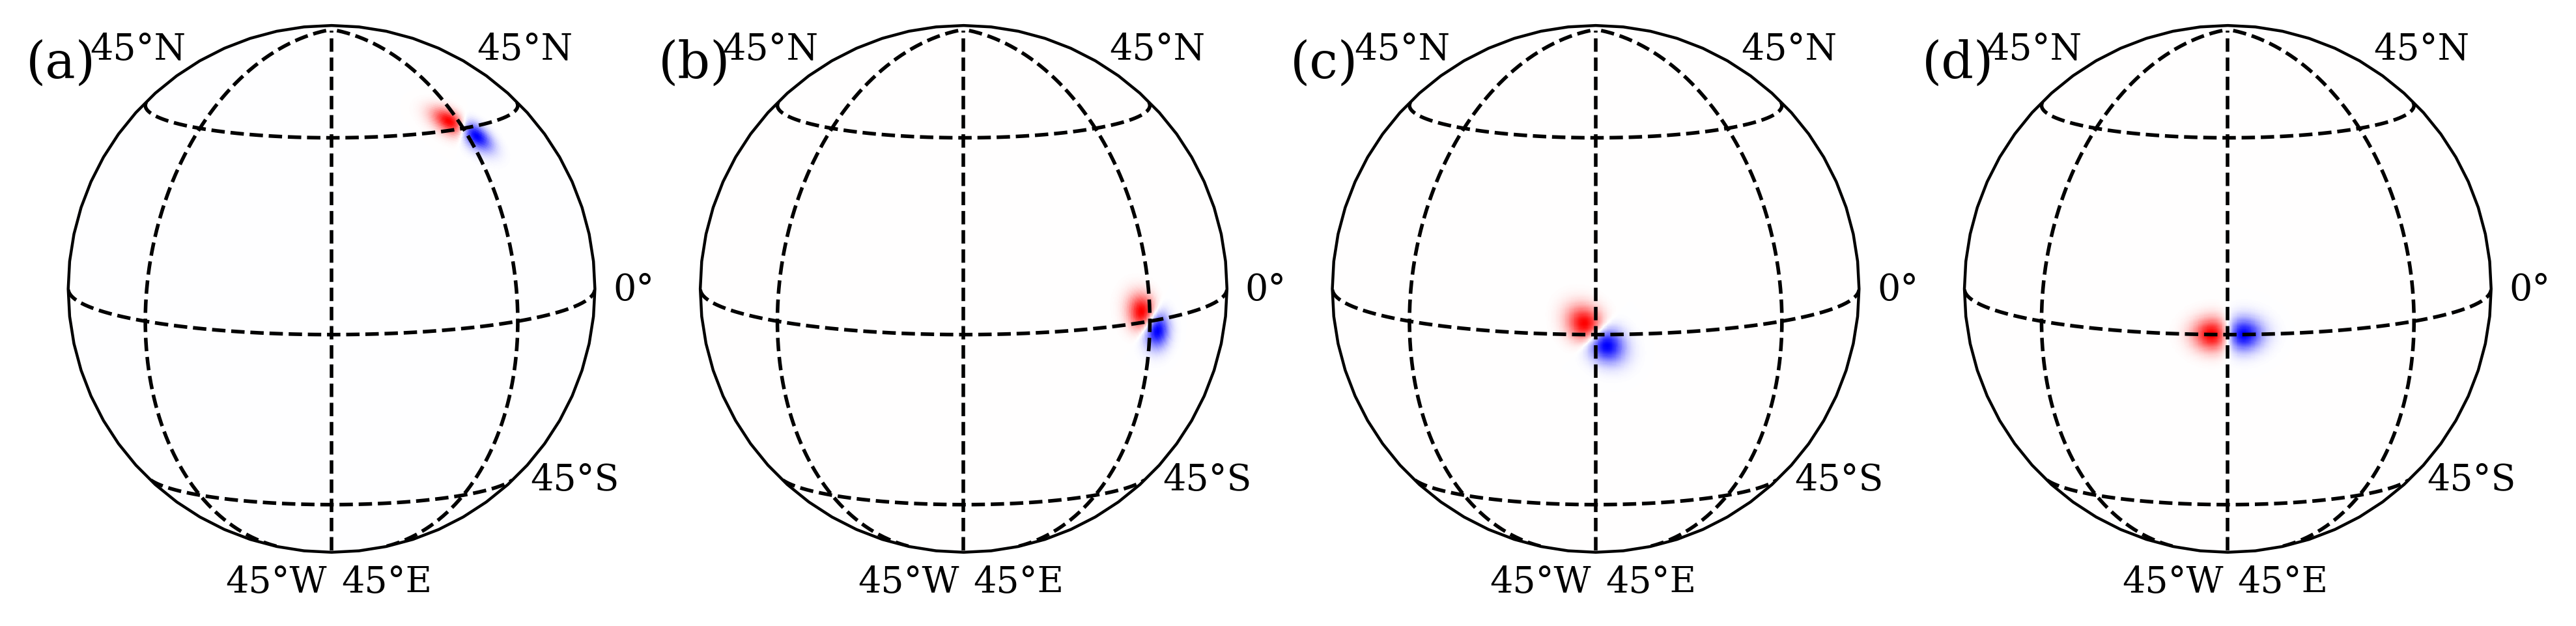
\includegraphics[width=0.85\textwidth]{assets/rotation_bmr.png}
    \caption{A BMR centered at 45$^{\circ}$ latitude and 45$^{\circ}$ longitude with a tilt of 45$^{\circ}$ with respect to the equator is shown in (a). Coordinate transformation operations along $\phi$,$\lambda$ and $\gamma$ are shown in (b), (c) and (d). The corresponding transformation matris is given by equation-\ref{eqn:rotation-trans}}
\end{figure}


%----------------------------------------------------------------------------------------
%	BIBLIOGRAPHY
%----------------------------------------------------------------------------------------

%\renewcommand{\refname}{\spacedlowsmallcaps{References}} % For modifying the bibliography heading

\bibliographystyle{assets/aasjournal}

\bibliography{assets/references.bib} % The file containing the bibliography

\end{document}
